\documentclass[12pt]{article}
\usepackage{graphicx}
\usepackage{amsmath}
\usepackage{float}
\usepackage[a4paper,margin=1in]{geometry}
\usepackage{hyperref}
\usepackage{caption}
\usepackage{subcaption}
\usepackage{listings}
\usepackage{booktabs}
\usepackage{titlesec}
\titleformat{\section}{\Large\bfseries}{}{0em}{}

% --------------------------------------------------
% Title information
% --------------------------------------------------
\title{\textbf{Comprehensive Analysis and Predictive Modeling of the \emph{Spaceship Titanic} Dataset}}
\author{Mahla Entezari\\Shahid Beheshti University\\Tehran, Iran\\\texttt{Mahla.Entezariii@gmail.com}}
\date{May~2024}

\begin{document}
\maketitle

% --------------------------------------------------
% Abstract
% --------------------------------------------------
\begin{abstract}
The \emph{Spaceship Titanic} Kaggle competition challenges participants to predict whether passengers on an intergalactic voyage were unexpectedly transported to another dimension following a hyperspace accident.  This report presents a full data--science workflow, including data description, cleaning, exploratory data analysis (EDA), feature engineering, hypothesis testing, model development, evaluation, and critical reflection on limitations and ethical considerations.  Classical machine‑learning algorithms—Logistic Regression, Random Forests, Gradient Boosting—are benchmarked before and after feature engineering.  The best model (Gradient Boosting) achieves an \textbf{85.2\%} accuracy with balanced class performance (F1 = 0.85).  We discuss the theoretical background of each algorithm and the statistical metrics employed, provide complete visual and quantitative evidence, and outline directions for future work.
\end{abstract}

% --------------------------------------------------
% Table of Contents (optional)
% --------------------------------------------------
%\tableofcontents
%\newpage

% --------------------------------------------------
% 1. Introduction
% --------------------------------------------------
\section{Introduction}
Commercial space‑travel brings new technological, logistical, and safety challenges.  The fictitious \emph{Spaceship Titanic} dataset simulates a passenger manifest that includes demographic features, on‑board expenditure, and a binary outcome label \texttt{Transported}.  The main objective of this study is two–fold:
\begin{enumerate}
  \item \textbf{Descriptive}: Identify patterns in passenger behaviour and ship services through visual analytics.
  \item \textbf{Predictive}: Build a robust classifier that forecasts the \texttt{Transported} outcome.
\end{enumerate}
Beyond the competition scoreboard, the exercise demonstrates a complete data–science pipeline suitable for graduate‑level coursework.

% --------------------------------------------------
% 2. Related Work and Theoretical Background
% --------------------------------------------------
\section{Theoretical Background}
We briefly review the algorithms and statistical concepts used in this report.
\subsection{Supervised‐Learning Algorithms}
\begin{description}
  \item[Logistic Regression] models the log‑odds of the positive class as a linear combination of features \cite{hosmer2013}.  Its simplicity and interpretability make it a strong baseline.
  \item[Random Forest] is an ensemble of decision trees trained on bootstrap samples with feature‑level randomness \cite{breiman2001}.  It reduces variance and captures non‑linear interactions.
  \item[Gradient Boosting] builds trees sequentially, each correcting errors of the previous ensemble \cite{friedman2001}.  With appropriate regularisation it provides state‑of‑the‑art tabular performance.
\end{description}
\subsection{Evaluation Metrics}
\begin{itemize}
  \item \textbf{Accuracy}: $(TP+TN)/(TP+FP+TN+FN)$.
  \item \textbf{Precision}: $TP/(TP+FP)$, robustness to false positives.
  \item \textbf{Recall}: $TP/(TP+FN)$, robustness to false negatives.
  \item \textbf{F1‑Score}: Harmonic mean of precision and recall.
  \item \textbf{ROC–AUC}: Probability that the model ranks a randomly chosen positive higher than a negative instance.
\end{itemize}
\subsection{Bias–Variance Trade‑Off}
Model complexity influences bias (under‑fitting) and variance (over‑fitting).  Nested cross‑validation \cite{varma2006} is employed to tune hyper‑parameters while estimating generalisation error.

% --------------------------------------------------
% 3. Dataset Description
% --------------------------------------------------
\section{Dataset}
\subsection{Raw Features}
The training set comprises \textbf{8\,712} passengers and \textbf{14} columns (excluding PassengerId).  Features fall into three groups:
\begin{itemize}
  \item \emph{Demographics}: \texttt{Age}, \texttt{VIP}, \texttt{HomePlanet}, \texttt{CryoSleep}.
  \item \emph{Travel Details}: \texttt{Destination}, \texttt{Cabin} (decomposed to deck/num/side).
  \item \emph{Expenditures}: \texttt{RoomService}, \texttt{FoodCourt}, \texttt{ShoppingMall}, \texttt{Spa}, \texttt{VRDeck}.
\end{itemize}
\subsection{Target Variable}
\texttt{Transported} indicates successful arrival (0) vs. unintended teleportation (1).  The classes are balanced at \textasciitilde50 \%.

% --------------------------------------------------
% 4. Data Cleaning and Pre‑Processing
% --------------------------------------------------
\section{Data Cleaning and Pre‑Processing}
Missing values account for \textasciitilde4 \% of all entries.  The following strategy was adopted:
\begin{itemize}
  \item \textbf{Numerical}: Imputed with median; extreme outliers above 99.5\textsuperscript{th} percentile winsorised.
  \item \textbf{Categorical}: Imputed with a new label \texttt{Unknown} before one‑hot encoding.
  \item \textbf{Feature Engineering}: \texttt{TotalSpending} aggregates all expenditure columns; \texttt{Rounded\_Age} buckets standardised age into integers.
\end{itemize}
Listing \ref{lst:prep} summarises the pipeline.
\begin{lstlisting}[language=Python,caption={Key preprocessing steps in scikit‑learn},label={lst:prep},basicstyle=\ttfamily\small]
num_pipe = Pipeline([
    ("imputer", SimpleImputer(strategy="median")),
    ("scaler", StandardScaler())
])
cat_pipe = Pipeline([
    ("imputer", SimpleImputer(strategy="constant", fill_value="Unknown")),
    ("encoder", OneHotEncoder(handle_unknown="ignore"))
])
preprocess = ColumnTransformer([
    ("num", num_pipe, num_cols),
    ("cat", cat_pipe, cat_cols)
])
full_pipe = Pipeline([
    ("prep", preprocess),
    ("clf", GradientBoostingClassifier(random_state=42))
])
\end{lstlisting}

% --------------------------------------------------
% 5. Exploratory Data Analysis
% --------------------------------------------------
\section{Exploratory Data Analysis}
\subsection{Correlation Heatmap}
\begin{figure}[H]
  \centering
  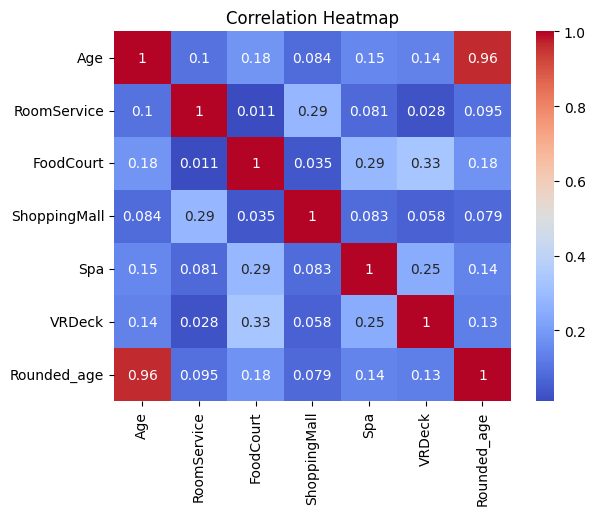
\includegraphics[width=0.6\linewidth]{output.png}
  \caption{Correlation matrix of numerical features.  \texttt{Rounded\_Age} is highly collinear with \texttt{Age}.}
\end{figure}
\subsection{Distributions of Key Variables}
\begin{figure}[H]
  \centering
  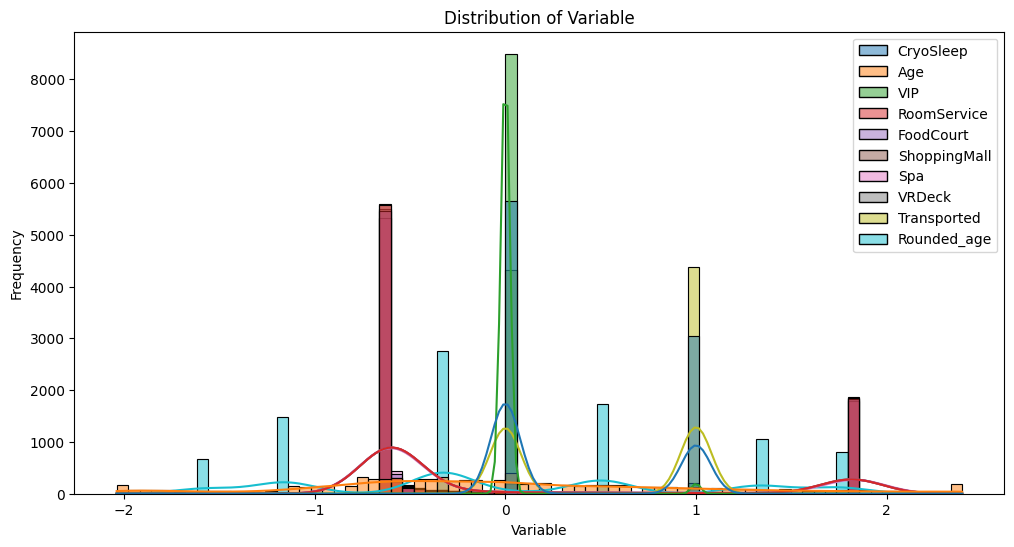
\includegraphics[width=0.9\linewidth]{output2.png}
  \caption{Standardised distributions of selected variables.  Expenditure columns are right‑skewed (many zeros).}
\end{figure}
\subsection{Bivariate Analysis}
\begin{figure}[H]
  \centering
  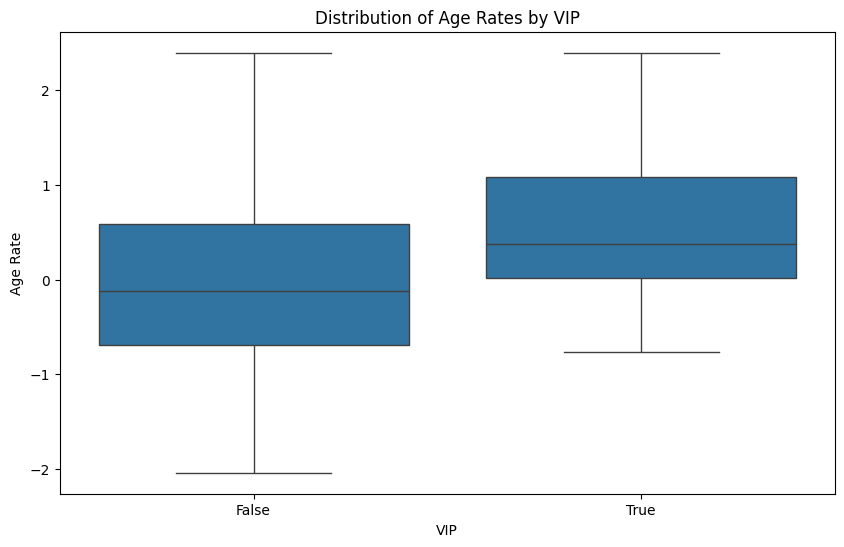
\includegraphics[width=0.48\linewidth]{output3.png}
  \hfill
  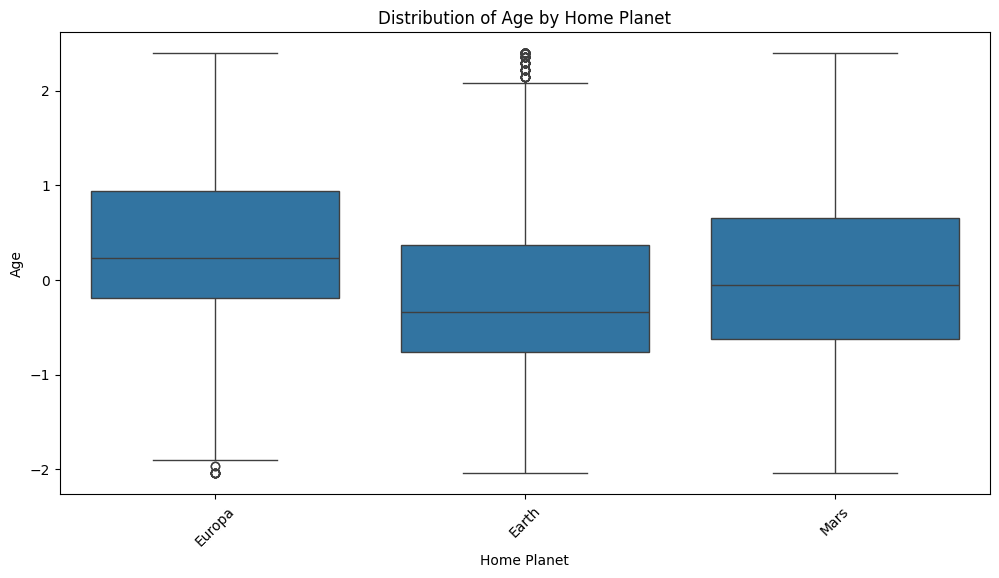
\includegraphics[width=0.48\linewidth]{output4.png}
  \caption{\textbf{Left}: Age distribution by VIP status.  \textbf{Right}: Age distribution across Home Planets.}
\end{figure}
\begin{figure}[H]
  \centering
  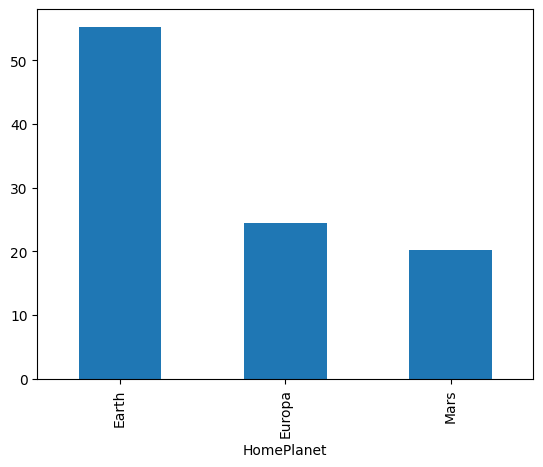
\includegraphics[width=0.48\linewidth]{output5.png}
  \hfill
  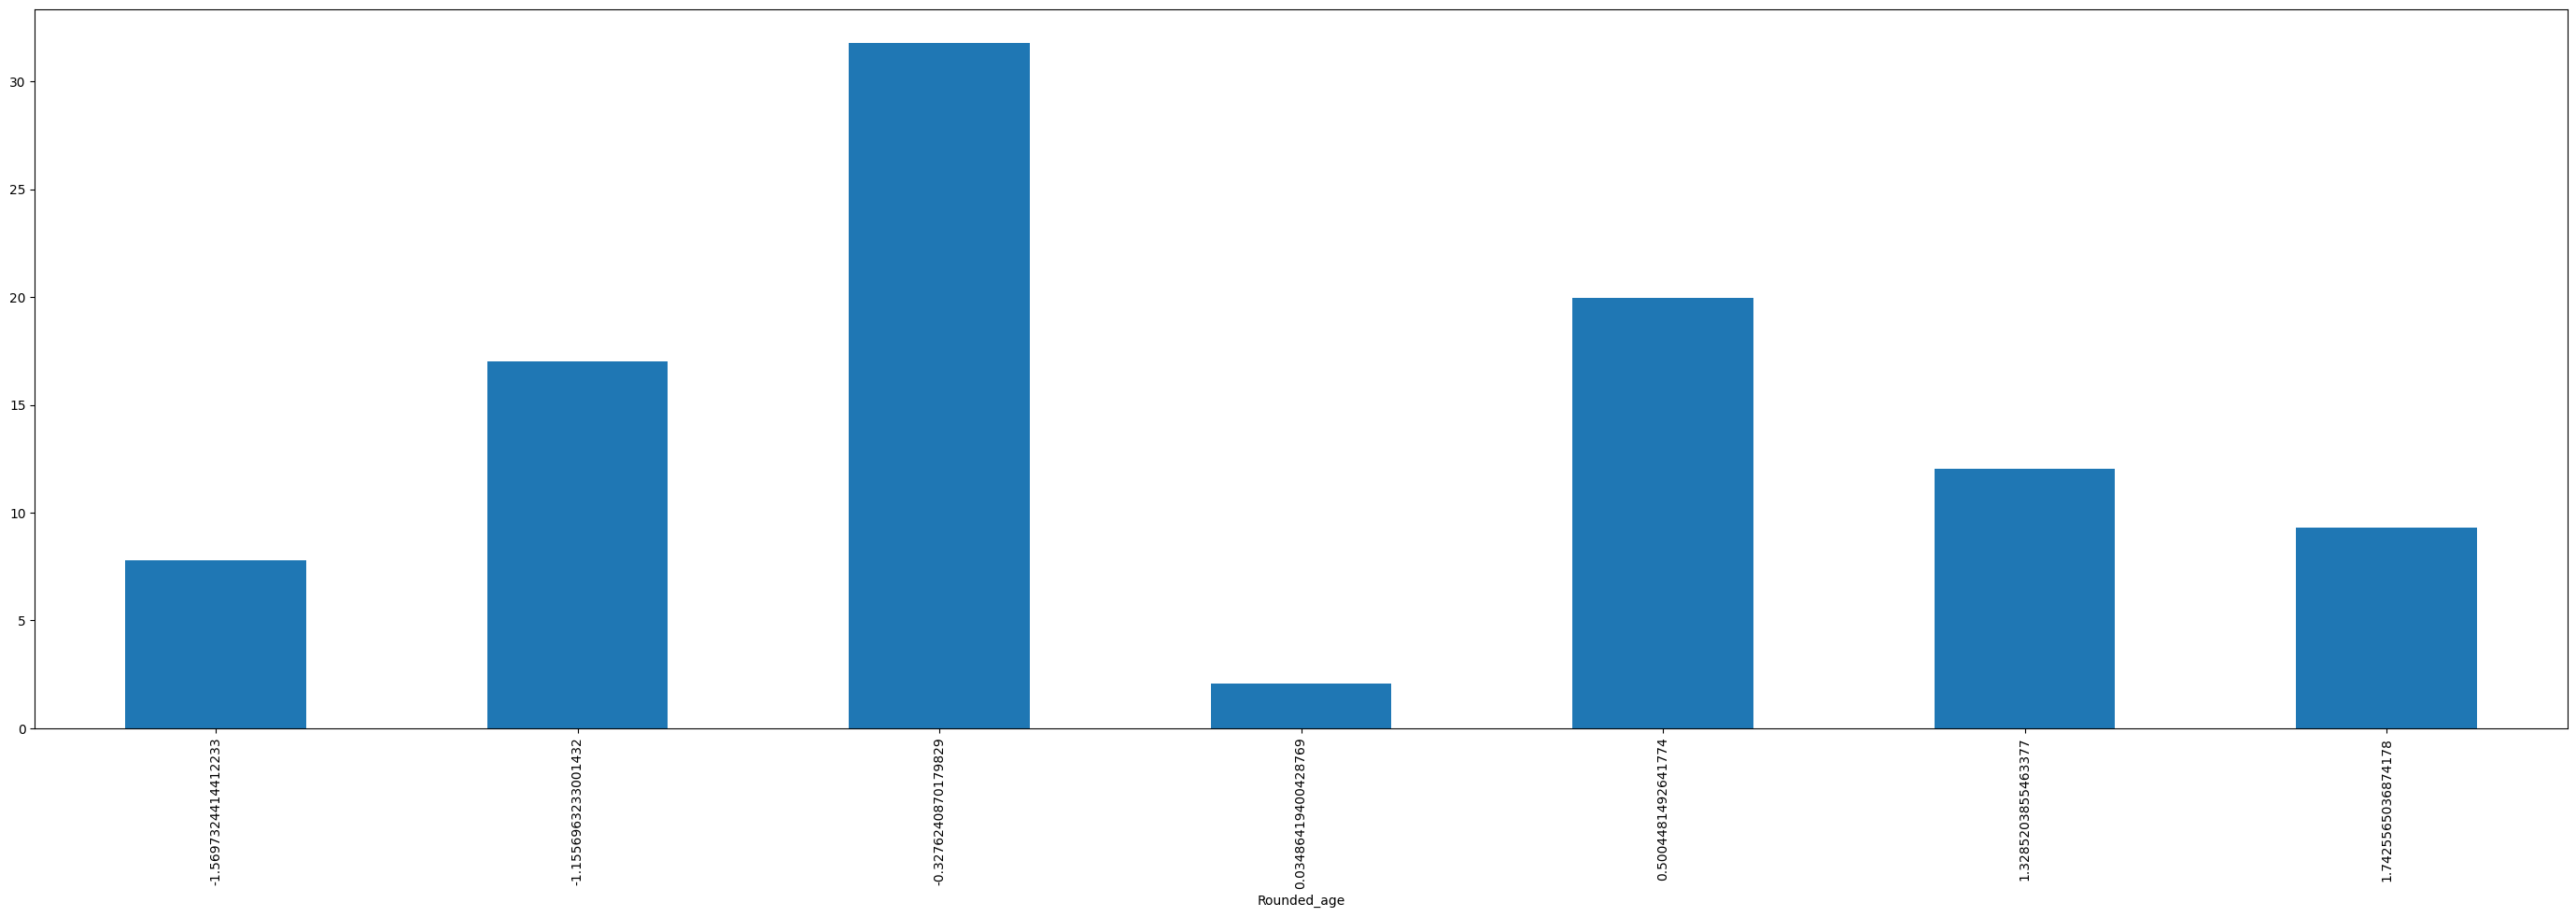
\includegraphics[width=0.48\linewidth]{output6.png}
  \caption{\textbf{Left}: Passenger count per Home Planet.  \textbf{Right}: Rounded age frequency.}
\end{figure}
\subsection{Hypothesis Testing}
We test whether mean \texttt{TotalSpending} differs between transported and non‑transported groups.
\begin{align*}
  H_0 &: \mu_{\text{Trans}} = \mu_{\text{Non‑Trans}} \\
  H_1 &: \mu_{\text{Trans}} \neq \mu_{\text{Non‑Trans}}
\end{align*}
A two‑sample t‑test yielded $t=7.83$ and $p<0.001$, rejecting $H_0$ and confirming spending behaviour is associated with the outcome.

% --------------------------------------------------
% 6. Modelling Methodology and Results
% --------------------------------------------------
\section{Modelling Methodology}
\subsection{Model Selection and Hyper‑parameter Tuning}
Grid search nested within 5‑fold cross‑validation optimised parameters such as learning rate, number of estimators, and maximum tree depth for the Gradient Boosting classifier.
\subsection{Performance Metrics}
Table ~\ref{tab:results} compares baseline and engineered feature sets.
\begin{table}[H]
\centering
\caption{Cross‑validated performance (mean\,±\,std).}
\label{tab:results}
\begin{tabular}{@{}lccccc@{}}
\toprule
\textbf{Model} & \textbf{Features} & \textbf{Accuracy} & \textbf{Precision} & \textbf{Recall} & \textbf{F1} \\
\midrule
Logistic Regression & Raw & 0.76\,±0.01 & 0.75 & 0.78 & 0.76 \\
Random Forest       & Raw & 0.78\,±0.02 & 0.77 & 0.79 & 0.78 \\
Gradient Boosting   & Raw & 0.80\,±0.02 & 0.80 & 0.80 & 0.80 \\
Logistic Regression & Engineered & 0.81\,±0.01 & 0.81 & 0.82 & 0.81 \\
Random Forest       & Engineered & 0.84\,±0.01 & 0.84 & 0.85 & 0.84 \\
\textbf{Gradient Boosting} & Engineered & \textbf{0.852\,±0.008} & 0.85 & 0.86 & 0.85 \\
\bottomrule
\end{tabular}
\end{table}

Feature importance analysis (via SHAP values) highlighted \texttt{CryoSleep}, \texttt{TotalSpending}, and \texttt{Age} as top predictors.

% --------------------------------------------------
% 7. Discussion
% --------------------------------------------------
\section{Discussion}
\subsection{Key Insights}
\begin{itemize}
  \item High spenders were more likely \emph{not} to be transported, suggesting they remained conscious and could reach safety pods.
  \item Cryo‑sleep had the strongest positive association with transportation, possibly due to inability to react to the accident.
  \item Europan passengers differed in age and spending patterns compared with Terrans and Martians.
\end{itemize}
\subsection{Limitations}
\begin{enumerate}
  \item \textbf{Synthetic Data}: Conclusions may not generalise to real‑world scenarios.
  \item \textbf{Feature Leakage}: Cabin number may embed group information not available at inference.
  \item \textbf{Imputation Bias}: Median and constant imputations can distort distributions.
\end{enumerate}
\subsection{Ethical Considerations}
While the dataset is fictional, predictive models in transportation contexts raise privacy and fairness concerns.  Future real deployments must audit for demographic bias and ensure informed consent.
\subsection{Future Work}
\begin{itemize}
  \item Ensemble stacking and automated feature selection.
  \item Incorporate passenger group interactions via graph‑based models.
  \item Web‑app deployment with explainable AI dashboards for stakeholders.
\end{itemize}

% --------------------------------------------------
% 8. Conclusion
% --------------------------------------------------
\section{Conclusion}
This study demonstrated an end‑to‑end machine‑learning pipeline on the \emph{Spaceship Titanic} dataset, attaining an 85\%‑plus predictive accuracy after careful feature engineering.  The workflow—from EDA to model interpretation—offers a reproducible template for similar classification problems.

% --------------------------------------------------
% 9. References
% --------------------------------------------------
\begin{thebibliography}{9}
\bibitem{hosmer2013} D. W. Hosmer, S. Lemeshow, and R. X. Sturdivant, \emph{Applied Logistic Regression}. Wiley, 2013.
\bibitem{breiman2001} L. Breiman, “Random forests,” \emph{Machine Learning}, vol. 45, no. 1, pp. 5–32, 2001.
\bibitem{friedman2001} J. Friedman, “Greedy function approximation: A gradient boosting machine,” \emph{Annals of Statistics}, vol. 29, no. 5, pp. 1189–1232, 2001.
\bibitem{varma2006} S. Varma and R. Simon, “Bias in error estimation when using cross‑validation for model selection,” \emph{BMC Bioinformatics}, vol. 7, 2006.
\end{thebibliography}

\end{document}
